\section{Chatbot Builder}

\subsection {Initial Design}
The Chatbot Builder is a web application that allows users to create chatbot workflows using a visual interface. This interface consists of a canvas where users can drag and drop nodes to create a flowchart-like structure. Each node represents a step in the chatbot conversation, and connections between nodes represent the flow of the conversation.

The following figure shows our initial design for the Chatbot Builder interface:

\begin{figure}[H]
    \centering
    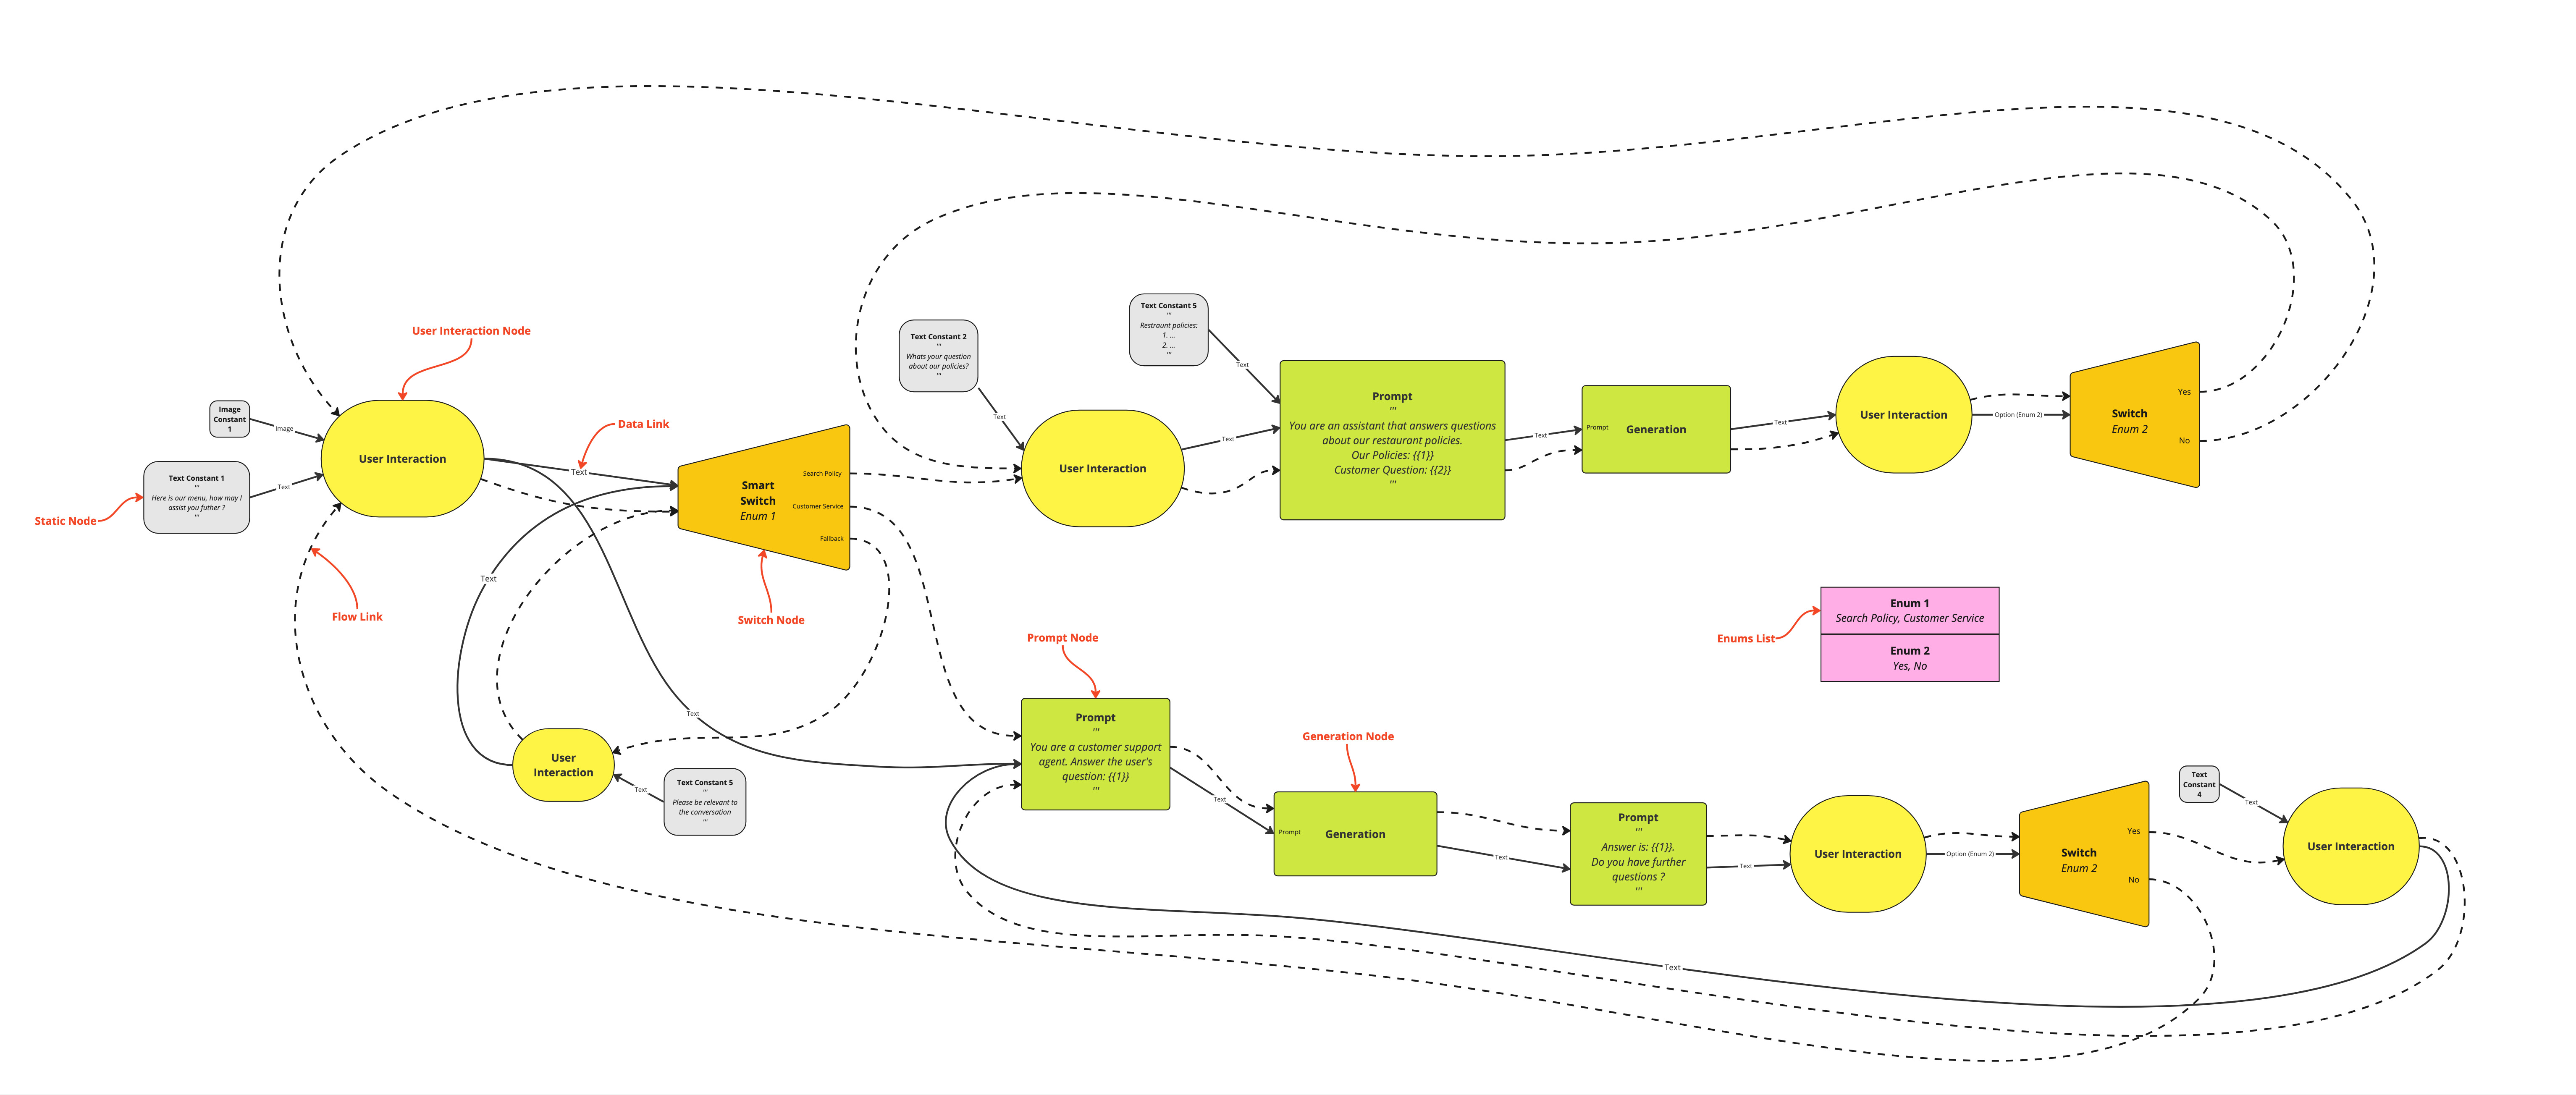
\includegraphics[width=0.95\textwidth]{assets/ChatbotBuilder_Sketch.jpg}
    \caption{Initial design of the Chatbot Builder interface}
    \label{fig:chatbot_builder}
\end{figure}

The design shows the following components:
\begin{itemize}
    \item \textbf{User Interaction Node}: Represents a user input node where the chatbot waits for user input.
    \item \textbf{Switch Node}: Represents a conditional node where the chatbot can branch based on a given option.
    \item \textbf{Prompt Node}: Represents a text template with placeholders for dynamic content at runtime.
    \item \textbf{Generation Node}: Represents a node that generates dynamic content using a language model.
    \item \textbf{Static Node}: Represents a constant value that is passed to other nodes.
    \item \textbf{Smart Switch Node}: Represents a conditional node that can branch based on the output of a language model, AKA Dynamic Routing.
    \item \textbf{Data Link}: Represents a connection between nodes that carries data from one node to another.
    \item \textbf{Flow Link}: Represents a connection between nodes that defines the flow of the conversation.
\end{itemize}


\subsection{Design Decisions}

\begin{itemize}
    \item In this design we had to add two types of links, Data Link and Flow Link, this is because data is not always passed between nodes in a linear fashion, sometimes data is passed between nodes that are not directly connected in the flow of the conversation.
    \item To ensure logical easy to understand design, we choose an Eager-Evaluation approach where the data is passed through data links as soon as the node finishes its execution. Lazy-Evaluation approach is hard to understand and debug, as the data is passed only when needed, which makes it hard to track the data flow.
    \item Also notice that in this design we have exactly one User node (Interaction Node) instead of separate Input and Output nodes, this is because the chatbot follows a request-response model, where the user sends a request and the chatbot responds with a message, so there won't be any case where the user input isn't followed directly.
\end{itemize}

\subsection{Conversation Flow}

\subsubsection{On Creation Request}
\begin{itemize}
    \item All static nodes are visited (In the order of their IDs), and their values are pushed through their output data links.
    \item Static nodes are of no use after that through out the whole conversation.
    \item Then the start (User Interaction) node is activated by returning output to  user in the response, then the server waits for the next request.
\end{itemize}

\subsubsection{On Further Requests}
\begin{itemize}
    \item Flow control resumes from the user interaction node which the server stopped on last time.
    \item User input is pushed through the node's output data links.
    \item Flow control moves to the next node through the node's flow link.
    \item The following nodes consecutively: activate, push their data, and move flow control. Until the server eventually hit another user interaction node.
    \item Output is finally returned to the user in the response. And the server waits for the next request.
\end{itemize} 
